\let\negmedspace\undefined
\let\negthickspace\undefined
\documentclass[journal]{IEEEtran}
\usepackage[a5paper, margin=10mm, onecolumn]{geometry}
\usepackage{lmodern} 
\usepackage{tfrupee} 
\setlength{\headheight}{1cm}
\setlength{\headsep}{0mm}   

\usepackage{gvv-book}
\usepackage{gvv}
\usepackage{cite}
\usepackage{amsmath,amssymb,amsfonts,amsthm}
\usepackage{algorithmic}
\usepackage{graphicx}
\usepackage{textcomp}
\usepackage{xcolor}
\usepackage{txfonts}
\usepackage{listings}
\usepackage{enumitem}
\usepackage{mathtools}
\usepackage{gensymb}
\usepackage{comment}
\usepackage[breaklinks=true]{hyperref}
\usepackage{tkz-euclide} 
\usepackage{listings}                             
\def\inputGnumericTable{}                                 
\usepackage[latin1]{inputenc}                                
\usepackage{color}                                            
\usepackage{array}                                            
\usepackage{longtable}                                       
\usepackage{calc}                                             
\usepackage{multirow}                                         
\usepackage{hhline}                                           
\usepackage{ifthen}                                           
\usepackage{lscape}
\usepackage{xparse}

\bibliographystyle{IEEEtran}

\title{4.13.66}
\author{EE25BTECH11062 - Vivek K Kumar}

\begin{document}
\maketitle

\renewcommand{\thefigure}{\theenumi}
\renewcommand{\thetable}{\theenumi}

\numberwithin{equation}{enumi}
\numberwithin{figure}{enumi} 

\textbf{Question}:\\
A straight line $L$ with negative slope passes through the point $\brak{8, 2}$ and cuts the
positive coordinate axes at points $P$ and $Q$. Find the absolute minimum value of
$OP + OQ$, as $L$ varies, where $O$ is the origin.

\textbf{Solution: }

\begin{table}[H]    
  \centering
  \begin{tabular}{|c|c|}
\hline
\textbf{Name} & \textbf{Value} \\ \hline
$\vec{A}$ & $\myvec{2 & 1 \\0 & 3}$ \\ \hline
\end{tabular}

  \caption{Variables used}
  \label{tab:4.13.66}
\end{table}

It is known that 
\begin{align}
    \vec{e_1}^\top\vec{P} = 0 \\
    \vec{e_2}^\top\vec{Q} = 0
\end{align}

Given line $L$ can be represented as 
\begin{align}
    \vec{x} = \vec{h} + k\vec{m} \\
    \vec{e_1}^\top\vec{P} = \vec{e_1}^\top\vec{h} + k_1\vec{e_1}^\top\vec{m} \\
    k_1 = -\frac{\vec{e_1}^\top\vec{h}}{\vec{e_1}^\top\vec{m}} \\
    \vec{P} = \vec{h} - \frac{\vec{e_1}^\top\vec{h}}{\vec{e_1}^\top\vec{m}}\vec{m} \\
    \vec{e_2}^\top\vec{Q} = \vec{e_2}^\top\vec{h} + k_2\vec{e_2}^\top\vec{m} \\
    k_2 = -\frac{\vec{e_2}^\top\vec{h}}{\vec{e_2}^\top\vec{m}} \\
    \vec{Q} = \vec{h} - \frac{\vec{e_2}^\top\vec{h}}{\vec{e_2}^\top\vec{m}}\vec{m} 
\end{align}

Substituting values
\begin{align}
    \vec{P} &= \myvec{8 \\ 2} - 8\myvec{1 \\ -m} \\
            &= \myvec{0 \\ 2+8m} \\
    \vec{Q} &= \myvec{8 \\ 2} - \frac{2}{m}\myvec{1 \\ -m} \\
            &= \myvec{8 + \frac{2}{m} \\ 0}
\end{align}
We have to find the minimum of $\norm{\vec{P}} + \norm{\vec{Q}}$
\begin{align}
    \norm{\vec{P}} + \norm{\vec{Q}} &= 2 + 8m + 8 + \frac{2}{m} \\
    &= 10 + 8m + \frac{2}{m}
\end{align}
Applying AM-GM inequality
\begin{align}
    \frac{8m + \frac{2}{m}}{2} &\geq \sqrt{8m .\frac{2}{m}} \\
    &\geq 4\\
    \implies 10 + 8m + \frac{2}{m} &\geq 18
\end{align}
Hence we can write
\begin{align}
    \norm{\vec{P}} + \norm{\vec{Q}} \geq 18
\end{align}
Hence, $min\brak{\norm{\vec{P}} + \norm{\vec{Q}}} = 18$

\begin{figure}[H]
   \centering
  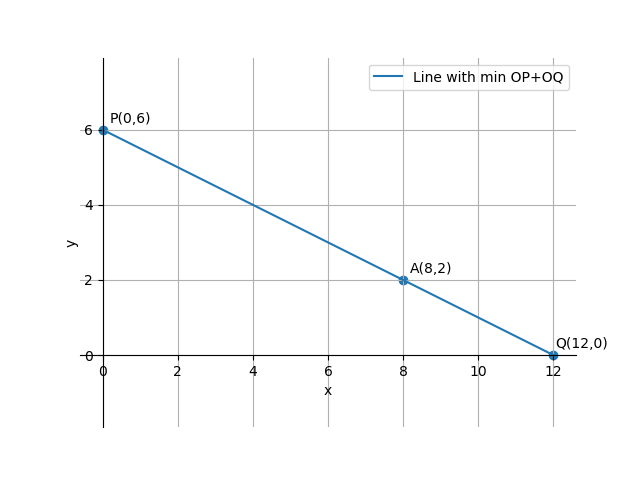
\includegraphics[width=0.64\columnwidth]{figs/fig.png}
   \caption{Given points on a line}
   \label{stemplot}
\end{figure}
\end{document}  